\documentclass{article}
\usepackage[utf8]{inputenc}

\usepackage{enumitem}
\usepackage{hyperref}
\usepackage{graphicx}
\usepackage{float}

\hypersetup{
    colorlinks=true,
    urlcolor=blue,
}

\title{TDT4305: Project Phase 1\\Exploratory Analysis of Twitter Dataset}
\author{Fredrik Bakken and Tor Arne Hagen}
\date{\today}

\begin{document}

\maketitle

\begin{figure}[H]
    \centering
    
\includegraphics[width=\textwidth]{PhaseOne/docs/img/big-data.png}
\end{figure}

\begin{figure}[H]
    \centering
    
\includegraphics[width=0.5\textwidth]{PhaseOne/docs/img/ntnu.png}
\end{figure}

\newpage

% QUESTION 1
\section*{Task 1: Load RDD and Explore}
\subsection*{Source Code and Results}
    \begin{itemize}
        \item \textbf{Source code:} task\_1.py (\href{https://github.com/FredrikBakken/TDT4305_Big-Data-Project/blob/master/PhaseOne/task_1.py}{Github})
        \item \textbf{Results:} /data/results/result\_1.tsv (\href{https://github.com/FredrikBakken/TDT4305_Big-Data-Project/blob/master/PhaseOne/data/results/result_1.tsv}{Github})
    \end{itemize}

\subsection*{Questions to be Answered}
\begin{enumerate}[label=\alph*)]
    % Question 1a
    \item \textit{How many tweets are there?}\\
    
    Total number of tweets: \textbf{2715066}.\\
    
    Solved by using the Spark function \textit{.count()} on the entire RDD data set.\\ \\
    
    
    % Question 1b
    \item \textit{How many distinct users (username) are there?}\\
    
    Number of distinct usernames: \textbf{499822}.\\
    
    Solved by using the Spark functions \textit{.map()}, \textit{.distinct()}, and \textit{.count()} on the USERNAME row of the data set.\\ \\
    
    
    % Question 1c
    \item \textit{How many distinct countries (country\_name) are there?}\\
    
    Number of distinct country names: \textbf{70}.\\
    
    Solved by using the Spark functions \textit{.map()}, \textit{.distinct()}, and \textit{.count()} on the COUNTRY\_NAME row of the data set.\\ \\
    
    
    % Question 1d
    \item \textit{How many distinct places (place\_name) are there?}\\
    
    Number of distinct place names: \textbf{23121}.\\
    
    Solved by using the Spark functions \textit{.map()}, \textit{.distinct()}, and \textit{.count()} on the PLACE\_NAME row of the data set.\\ \\
    
    
    % Question 1e
    \item \textit{In how many languages users post tweets?}\\
    
    Number of distinct languages: \textbf{46}.\\
    
    Solved by using the Spark functions \textit{.map()}, \textit{.distinct()}, and \textit{.count()} on the LANGUAGE row of the data set.\\ \\
    
    
    % Question 1f
    \item \textit{What is the minimum latitude?}\\
    
    Minimum latitude: \textbf{-54.87555556}.\\
    
    Solved by using the Spark function \textit{.min()} on the LATITUDE row of the data set.\\ \\
    
    
    % Question 1g
    \item \textit{What is the minimum longitude?}\\
    
    Minimum longitude: \textbf{-159.83019441}.\\
    
    Solved by using the Spark function \textit{.min()} on the LONGITUDE row of the data set.\\ \\
    
    
    % Question 1h
    \item \textit{What is the maximum latitude?}\\
    
    Maximum latitude: \textbf{69.83186826}.\\
    
    Solved by using the Spark function \textit{.max()} on the LATITUDE row of the data set.\\ \\
    
    
    % Question 1i
    \item \textit{What is the maximum longitude?}\\
    
    Maximum longitude: \textbf{153.03508445}.\\
    
    Solved by using the Spark function \textit{.max()} on the LONGITUDE row of the data set.\\ \\
    
    
    % Question 1j
    \item \textit{ What is the average length of a tweet text in terms of characters?}\\
    
    Average number of characters in each tweet: \textbf{87.2014098368}.\\
    
    Solved by using the Spark functions \textit{.map()} and \textit{.mean()} on the length of the TWEET\_TEXT row of the data set.\\ \\
    
    
    % Question 1k
    \item \textit{What is the average length of a tweet text in terms of words?}\\
    
    Average number of words in each tweet: \textbf{12.2284228081}.\\
    
    Solved by using the Spark functions \textit{.map()} and \textit{.mean()} on the split (by empty space) length of the TWEET\_TEXT row of the data set.\\ \\
\end{enumerate}


% QUESTION 2
\section*{Task 2: Tweet Counts per Country}
\subsection*{Source Code and Results}
    \begin{itemize}
        \item \textbf{Source code:} task\_2.py (\href{https://github.com/FredrikBakken/TDT4305_Big-Data-Project/blob/master/PhaseOne/task_2.py}{Github})
        \item \textbf{Results:} /data/results/result\_2.tsv (\href{https://github.com/FredrikBakken/TDT4305_Big-Data-Project/blob/master/PhaseOne/data/results/result_2.tsv}{Github})
    \end{itemize}

\subsection*{Questions to be Answered}
\begin{enumerate}[label=\alph*)]
    \item \textit{Find the total number of tweets posted from each country and sort them in descending order of tweet counts. For countries with equal number of tweets, sorting must be in alphabetical order.}\\
    
    To solve task 2, the tweets are first mapped by the origin country before they are counted. The output items are then sorted by the built-in Python method for sorting elements, where the tweet count is sorted in descending order and the countries with the same amount of tweets are sorted in alphabetic order.\\ \\
\end{enumerate}
\newpage

% QUESTION 3
\section*{Task 3: Geographical Centroids per Country}
\subsection*{Source Code and Results}
    \begin{itemize}
        \item \textbf{Source code:} task\_3.py (\href{https://github.com/FredrikBakken/TDT4305_Big-Data-Project/blob/master/PhaseOne/task_3.py}{Github})
        \item \textbf{Results:} /data/results/result\_3.tsv (\href{https://github.com/FredrikBakken/TDT4305_Big-Data-Project/blob/master/PhaseOne/data/results/result_3.tsv}{Github})
    \end{itemize}

\subsection*{Questions to be Answered}
\begin{enumerate}[label=\alph*)]
    \item \textit{Write a code (named "task\_3") that outputs in a TSV file the latitude and longitude of the centroids and the names of the countries, in the form of \textless country\_name\textgreater tab\textless latitude\textgreater tab\textless longitude\textgreater .}\\
    
    The final code solution in task 3 uses a method which creates an extreme run-time of more 30min. Eventhough the execution time is extremely slow because of so many Spark tasks, it still gives the correct result.\\
    
    A more efficient solution would take advantage of the aggregation method.\\
    
    \item \textit{Visualize the results in CartoDB.}\\
    
    \begin{figure}[H]
        \centering
        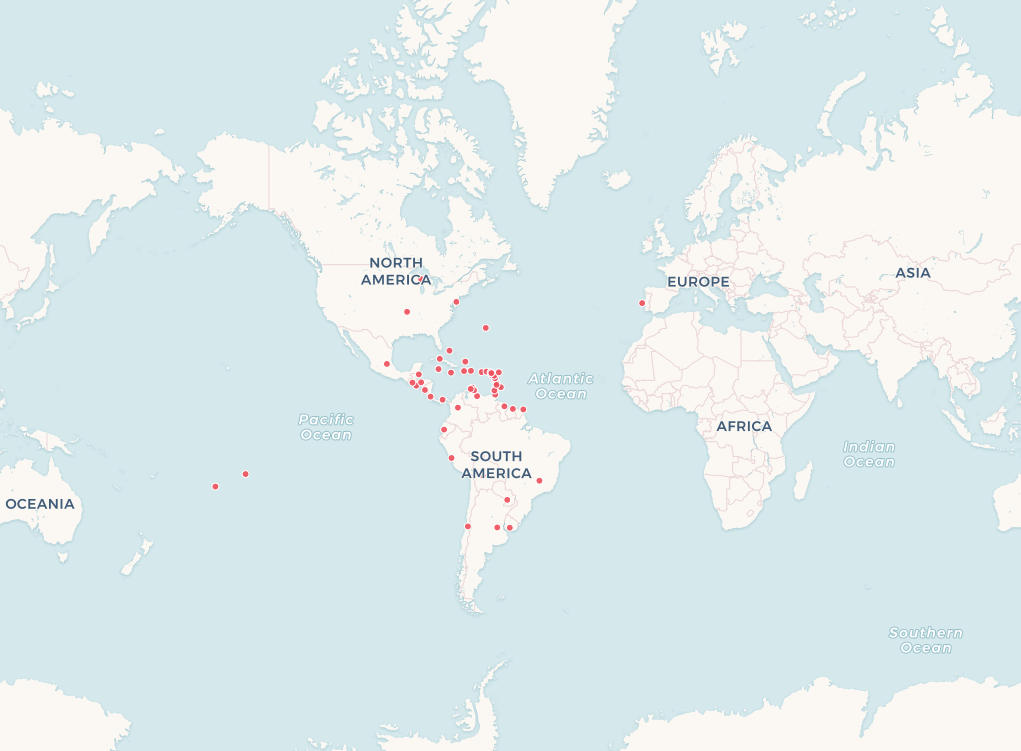
\includegraphics[width=11.9cm]{PhaseOne/docs/img/cartodb-visualization.png}
        \caption{Result Visualization in CartoDB.}
        \label{fig:cartodb}
    \end{figure}
    
\end{enumerate}


% QUESTION 4
\section*{Task 4: Most Active Hours per Country}
\subsection*{Source Code and Results}
    \begin{itemize}
        \item \textbf{Source code:} task\_4.py (\href{https://github.com/FredrikBakken/TDT4305_Big-Data-Project/blob/master/PhaseOne/task_4.py}{Github})
        \item \textbf{Results:} /data/results/result\_4.tsv (\href{https://github.com/FredrikBakken/TDT4305_Big-Data-Project/blob/master/PhaseOne/data/results/result_4.tsv/part-00000}{Github})
    \end{itemize}

\subsection*{Questions to be Answered}
\begin{enumerate}[label=\alph*)]
    \item \textit{Calculate local time for each tweet (UTC time + timezone offset) and find the 1-hour interval with maximum number of tweets for each country in the form of \textless country\_name\textgreater tab\textless begining\_hour\textgreater tab\textless tweet\_count\textgreater 3. Times should be rounded down to the hour, in 24 hour scale, so that a tweet posted between [13:00,14:00) should be interpreted as posted at 13. Write a code (named "task\_4") that writes the results in a TSV file and name it "result\_4.tsv".}\\
    
    In task 4, one starts by mapping the tweets by COUNTRY\_NAME, UTC\_TIME, and TIMEZONE\_OFFSET, where the two time rows are added together. Then the total time is transformed to actual hour-based time using the datetime library. Next, tweets for each hour for every country is counted and compared to find the hour where most tweets are posted for each country.\\ \\
\end{enumerate}


% QUESTION 5
\section*{Task 5: Tweet Counts per City}
\subsection*{Source Code and Results}
    \begin{itemize}
        \item \textbf{Source code:} task\_5.py (\href{https://github.com/FredrikBakken/TDT4305_Big-Data-Project/blob/master/PhaseOne/task_5.py}{Github})
        \item \textbf{Results:} /data/results/result\_5.tsv (\href{https://github.com/FredrikBakken/TDT4305_Big-Data-Project/blob/master/PhaseOne/data/results/result_5.tsv}{Github})
    \end{itemize}

\subsection*{Questions to be Answered}
\begin{enumerate}[label=\alph*)]
    \item \textit{Find the number of tweets from each city in US (place\_type = "city" and country\_code = "US") in the form of \textless place\_name\textgreater tab\textless tweet\_count\textgreater. Write a code (named "task\_5" that writes the results in a TSV file named "result\_5.tsv" in descending order of tweet counts. For cities with equal number of tweets, sorting must be in alphabetical order.}\\
    
    In task 5, one first filters the tweets by the COUNTRY\_CODE 'US' and PLACE\_TYPE 'city'. Then, each PLACE\_NAME is mapped with a value, before they are added together and sorted in descending order.\\ \\
\end{enumerate}


% QUESTION 6
\section*{Task 6: Frequent Words in a Country}
\subsection*{Source Code and Results}
    \begin{itemize}
        \item \textbf{Source code:} task\_6.py (\href{https://github.com/FredrikBakken/TDT4305_Big-Data-Project/blob/master/PhaseOne/task_6.py}{Github})
        \item \textbf{Results:} /data/results/result\_6.tsv (\href{https://github.com/FredrikBakken/TDT4305_Big-Data-Project/blob/master/PhaseOne/data/results/result_6.tsv}{Github})
    \end{itemize}

\subsection*{Questions to be Answered}
\begin{enumerate}[label=\alph*)]
    \item \textit{Find the 10 most frequent words (in lowercase) and their frequencies from the US, excluding the words shorter than 2 characters (length \textless 2) and the words from the stop words file. Write a code (named "task\_6") that writes the results in a TSV file named "result\_6.tsv" in the form of \textless word\textgreater tab\textless frequency\textgreater.}\\
    
    To solve this task, one first reads the stop words from the stop\_words.tsv file and appends all the words to a list. Thereafter, processing of the tweets start by filteringer on the COUNTRY\_CODE 'US'. All words TWEET\_TEXTs are then set to lowercase and split to lists, before stop words and short words are filtered out. The words that are left are now mapped with (word, 1), to represent the count for each word. ReduceByKey is then used to count the total instances of each word, before sorting the words by their count in descending order. The 10 most used words are then taken out of the result and appended to result\_6.tsv.\\ \\
\end{enumerate}


% QUESTION 7
\section*{Task 7: Frequent Words per City}
\subsection*{Source Code and Results}
    \begin{itemize}
        \item \textbf{Source code:} task\_7.py (\href{https://github.com/FredrikBakken/TDT4305_Big-Data-Project/blob/master/PhaseOne/task_7.py}{Github})
        \item \textbf{Results:} /data/results/result\_7.tsv (\href{https://github.com/FredrikBakken/TDT4305_Big-Data-Project/blob/master/PhaseOne/data/results/result_7.tsv}{Github})
    \end{itemize}

\subsection*{Questions to be Answered}
\begin{enumerate}[label=\alph*)]
    \item \textit{Find the 5 cities in the US with the highest number of tweets (place\_type = "city" and country\_code = "US", ordered by their tweet counts/alphabetical). For these 5 cities, find the 10 most frequent words ordered by their frequency, ignoring the stop words from the file and excluding words shorted than 2 characters (length \textless 2). Write a code (named "task\_7") that writes the results in a TSV file named "result\_7.tsv" in the form of \textless place\_name\textgreater \\
    tab\textless word1\textgreater tab\textless frequency1\textgreater tab\textless word2\textgreater tab\textless frequency2\textgreater ... \textless word10\textgreater \\
    tab\textless frequency10\textgreater .}\\
    
    In task 7 one first finds the top 5 cities in the US by filtering on COUNTRY\_NAME and PLACE\_TYPE, before mapping each place with a value. Then reducebykey and sorting in descending order is used to find the top 5 cities. Afterwards, a loop is initiated for loop through each of the cities to find each of their top 10 words as was done in task 6.\\ \\
\end{enumerate}


% QUESTION 8
\section*{Task 8: Explore using Spark SQL and Dataset API}
\subsection*{Source Code and Results}
    \begin{itemize}
        \item \textbf{Source code:} task\_8.py (\href{https://github.com/FredrikBakken/TDT4305_Big-Data-Project/blob/master/PhaseOne/task_8.py}{Github})
        \item \textbf{Results:} /data/results/result\_8.tsv (\href{https://github.com/FredrikBakken/TDT4305_Big-Data-Project/blob/master/PhaseOne/data/results/result_8.jpg}{Github})
    \end{itemize}

\subsection*{Questions to be Answered}
\begin{enumerate}[label=\alph*)]
    \item \textit{Number of tweets?}\\
    
    Total number of tweets: \textbf{2715066}.\\
    
    Solved by using the Spark SQL function \textit{.count()}.\\
    
    \item \textit{Number of distinct users (username)?}\\
    
    Number of distinct usernames: \textbf{499822}.\\
    
    Solved by using the Spark SQL functions \textit{.count()} and  \textit{.distinct()}.\\
    
    \item \textit{Number of distinct countries (country name)?}\\
    
    Number of distinct country names: \textbf{70}.\\
    
    Solved by using the Spark SQL functions \textit{.count()} and  \textit{.distinct()}.\\
    
    \item \textit{Number of distinct places (place name)?}\\
    
    Number of distinct place names: \textbf{23121}.\\
    
    Solved by using the Spark SQL functions \textit{.count()} and  \textit{.distinct()}.\\
    
    \item \textit{Number of distinct languages users post tweets?}\\
    
    Number of distinct languages: \textbf{46}.\\
    
    Solved by using the Spark SQL functions \textit{.count()} and  \textit{.distinct()}.\\
    
    \item \textit{Minimum values of latitude and longitude?}\\
    
    Minimum latitude: \textbf{-54.87555556}.\\
    Minimum longitude: \textbf{-159.83019441}.\\
    
    Solved by using the Spark SQL function \textit{.min()}.\\
    
    \item \textit{Maximum values of latitude and longitude?}\\
    
    Maximum latitude: \textbf{69.83186826}.\\
    Maximum longitude: \textbf{153.03508445}.\\
    
    Solved by using the Spark SQL function \textit{.max()}.\\
\end{enumerate}

\end{document}